\documentclass[tikz,border=0pt]{standalone}
\usepackage{xcolor}
\usetikzlibrary{calc}
% Palette: Sam_Comm_final.png by eye, and the drones and raiders.
\definecolor{ink}{HTML}{3B2340}
\definecolor{sky}{HTML}{EFC46A}
\definecolor{skyhi}{HTML}{F5DA92}
\definecolor{skylow}{HTML}{E9B060}
\definecolor{cloud}{HTML}{F2D58A}
\definecolor{paper}{HTML}{FBEFD0}
\definecolor{cream}{HTML}{FFF6E0}
\definecolor{white}{HTML}{FFFFFF}
\definecolor{wallA}{HTML}{E88A73}
\definecolor{wallB}{HTML}{EE9F7E}
\definecolor{wallC}{HTML}{E47A7E}
\definecolor{wallD}{HTML}{F0B07E}
\definecolor{wallE}{HTML}{D9765F}
\definecolor{wallF}{HTML}{E99A8A}
\definecolor{greenA}{HTML}{8DBB7E}
\definecolor{greenB}{HTML}{6FA77A}
\definecolor{greenC}{HTML}{A9C97F}
\definecolor{greenD}{HTML}{5E9C6A}
\definecolor{greenE}{HTML}{4A8060}
\definecolor{sage}{HTML}{9DB98A}
\definecolor{sagedark}{HTML}{6F8F66}
\definecolor{sagelight}{HTML}{C2D6A6}
\definecolor{window}{HTML}{F6E7A0}
\definecolor{windark}{HTML}{8C5A64}
\definecolor{metal}{HTML}{8D9A93}
\definecolor{metaldark}{HTML}{5E6B66}
\definecolor{metallight}{HTML}{B9C4BC}
\definecolor{wood}{HTML}{B9835A}
\definecolor{wooddark}{HTML}{8C5A3C}
\definecolor{woodlight}{HTML}{D9A66F}
\definecolor{stone}{HTML}{E7C9A0}
\definecolor{stonedark}{HTML}{C9A47E}
\definecolor{concrete}{HTML}{D8C3A4}
\definecolor{concretedark}{HTML}{B8A084}
\definecolor{asphalt}{HTML}{8E7A86}
\definecolor{asphaltdark}{HTML}{6E5C68}
\definecolor{roadline}{HTML}{F6E7A0}
\definecolor{kerb}{HTML}{D8B48C}
\definecolor{red}{HTML}{E0483E}
\definecolor{redlight}{HTML}{F27A6A}
\definecolor{gold}{HTML}{FFB000}
\definecolor{goldlight}{HTML}{FFD54F}
\definecolor{teal}{HTML}{4FA3A0}
\definecolor{tealdark}{HTML}{3C8582}
\definecolor{magenta}{HTML}{FF2E88}
\definecolor{cyan}{HTML}{13CFE3}
\definecolor{violet}{HTML}{8A5BD6}
\definecolor{orange}{HTML}{F2803A}
\definecolor{pink}{HTML}{F48FB1}
\definecolor{glow}{HTML}{4FE6E0}
\definecolor{glowhi}{HTML}{C8FFF9}
\definecolor{hot}{HTML}{FF6A1A}
\definecolor{hothi}{HTML}{FFD07A}
\definecolor{armour}{HTML}{7E7A86}
\definecolor{armourdark}{HTML}{5A5466}
\definecolor{armourlight}{HTML}{A8A2B0}
\definecolor{wasp}{HTML}{E0A82E}
\definecolor{waspdark}{HTML}{B07E1A}
\definecolor{moth}{HTML}{F2E6C8}
\definecolor{mothdark}{HTML}{D2C09A}
\definecolor{hornet}{HTML}{3C8582}
\definecolor{hornetdark}{HTML}{2C6260}
\definecolor{warden}{HTML}{E47A7E}
\definecolor{wardendark}{HTML}{B85A62}
\definecolor{tick}{HTML}{8DBB7E}
\definecolor{tickdark}{HTML}{5E8A5A}
\definecolor{strider}{HTML}{D9765F}
\definecolor{striderdark}{HTML}{A8543F}
\definecolor{jacket}{HTML}{6FA77A}
\definecolor{jacketb}{HTML}{4FA3A0}
\definecolor{jacketc}{HTML}{E88A73}
\definecolor{jacketd}{HTML}{F0B07E}
\definecolor{skin}{HTML}{F2C49A}
\definecolor{skinb}{HTML}{C98C6A}
\definecolor{skinc}{HTML}{8C5A3C}
\definecolor{hair}{HTML}{3B2340}
\definecolor{goo}{HTML}{B6E35A}
\definecolor{goodark}{HTML}{7FB23A}
\newcommand{\Ink}{1.8pt}
\tikzset{inked/.style={draw=ink, line width=\Ink, line join=round, line cap=round}}
\begin{document}
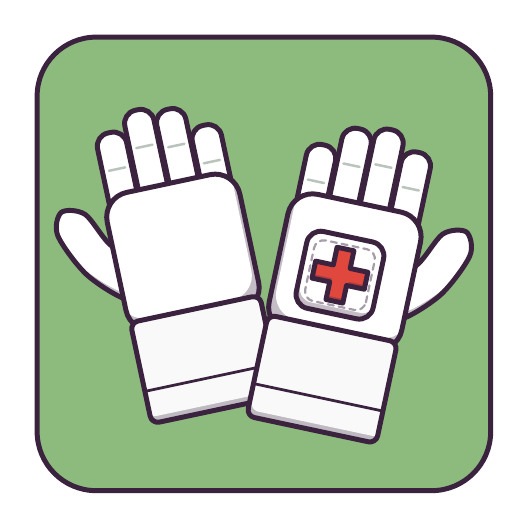
\begin{tikzpicture}
\clip (0,0) rectangle (6,6);
\fill[greenA] [rounded corners=0.75cm] (0.12,0.12) rectangle (5.88,5.88);
\begin{scope}\clip [rounded corners=0.75cm] (0.12,0.12) rectangle (5.88,5.88);
\begin{scope}[shift={(1.95,3.25)}, rotate=12, xscale=1.05, yscale=1.05]
\begin{scope}\clip plot[smooth cycle, tension=0.5] coordinates {(-0.703,-0.547) (-1.178,-0.146) (-1.438,0.406) (-1.339,0.678) (-1.062,0.594) (-0.822,0.146) (-0.397,-0.153)};
\fill[white!70!ink] plot[smooth cycle, tension=0.5] coordinates {(-0.703,-0.547) (-1.178,-0.146) (-1.438,0.406) (-1.339,0.678) (-1.062,0.594) (-0.822,0.146) (-0.397,-0.153)};
\fill[white, shift={(-0.035,0.1)}] plot[smooth cycle, tension=0.5] coordinates {(-0.703,-0.547) (-1.178,-0.146) (-1.438,0.406) (-1.339,0.678) (-1.062,0.594) (-0.822,0.146) (-0.397,-0.153)};
\end{scope}
\draw[inked] plot[smooth cycle, tension=0.5] coordinates {(-0.703,-0.547) (-1.178,-0.146) (-1.438,0.406) (-1.339,0.678) (-1.062,0.594) (-0.822,0.146) (-0.397,-0.153)};
\begin{scope}\clip[rounded corners=0.17cm] (-0.75,0.3) rectangle (-0.39,1.5);
\fill[white!70!ink,rounded corners=0.17cm] (-0.75,0.3) rectangle (-0.39,1.5);
\fill[white,rounded corners=0.17cm, shift={(-0.028,0.08)}] (-0.75,0.3) rectangle (-0.39,1.5);
\end{scope}
\draw[inked,rounded corners=0.17cm] (-0.75,0.3) rectangle (-0.39,1.5);
\draw[metallight, line width=0.9pt, line cap=round] (-0.67,1.05) -- (-0.47,1.05);
\begin{scope}\clip[rounded corners=0.17cm] (-0.37,0.3) rectangle (-0.01,1.7);
\fill[white!70!ink,rounded corners=0.17cm] (-0.37,0.3) rectangle (-0.01,1.7);
\fill[white,rounded corners=0.17cm, shift={(-0.028,0.08)}] (-0.37,0.3) rectangle (-0.01,1.7);
\end{scope}
\draw[inked,rounded corners=0.17cm] (-0.37,0.3) rectangle (-0.01,1.7);
\draw[metallight, line width=0.9pt, line cap=round] (-0.29,1.25) -- (-0.09,1.25);
\begin{scope}\clip[rounded corners=0.17cm] (0.01,0.3) rectangle (0.37,1.63);
\fill[white!70!ink,rounded corners=0.17cm] (0.01,0.3) rectangle (0.37,1.63);
\fill[white,rounded corners=0.17cm, shift={(-0.028,0.08)}] (0.01,0.3) rectangle (0.37,1.63);
\end{scope}
\draw[inked,rounded corners=0.17cm] (0.01,0.3) rectangle (0.37,1.63);
\draw[metallight, line width=0.9pt, line cap=round] (0.09,1.18) -- (0.29,1.18);
\begin{scope}\clip[rounded corners=0.17cm] (0.39,0.3) rectangle (0.75,1.35);
\fill[white!70!ink,rounded corners=0.17cm] (0.39,0.3) rectangle (0.75,1.35);
\fill[white,rounded corners=0.17cm, shift={(-0.028,0.08)}] (0.39,0.3) rectangle (0.75,1.35);
\end{scope}
\draw[inked,rounded corners=0.17cm] (0.39,0.3) rectangle (0.75,1.35);
\draw[metallight, line width=0.9pt, line cap=round] (0.47,0.9) -- (0.67,0.9);
\begin{scope}\clip[rounded corners=0.32cm] (-0.82,-0.95) rectangle (0.82,0.75);
\fill[white!70!ink,rounded corners=0.32cm] (-0.82,-0.95) rectangle (0.82,0.75);
\fill[white,rounded corners=0.32cm, shift={(-0.056,0.16)}] (-0.82,-0.95) rectangle (0.82,0.75);
\end{scope}
\draw[inked,rounded corners=0.32cm] (-0.82,-0.95) rectangle (0.82,0.75);
\begin{scope}\clip[rounded corners=0.1cm] (-0.8,-2.05) rectangle (0.8,-0.8);
\fill[white!90!metallight!70!ink,rounded corners=0.1cm] (-0.8,-2.05) rectangle (0.8,-0.8);
\fill[white!90!metallight,rounded corners=0.1cm, shift={(-0.028,0.08)}] (-0.8,-2.05) rectangle (0.8,-0.8);
\end{scope}
\draw[inked,rounded corners=0.1cm] (-0.8,-2.05) rectangle (0.8,-0.8);
\draw[ink, line width=1.0pt] (-0.8,-1.65) -- (0.8,-1.65);
\draw[white, line width=2pt, line cap=round, line join=round, opacity=0.8] plot[smooth, tension=0.6] coordinates {(-0.55,-0.4) (-0.55,0.45)};
\end{scope}
\begin{scope}[shift={(4.05,3)}, rotate=-12, xscale=-1.05, yscale=1.05]
\begin{scope}\clip plot[smooth cycle, tension=0.5] coordinates {(-0.703,-0.547) (-1.178,-0.146) (-1.438,0.406) (-1.339,0.678) (-1.062,0.594) (-0.822,0.146) (-0.397,-0.153)};
\fill[white!70!ink] plot[smooth cycle, tension=0.5] coordinates {(-0.703,-0.547) (-1.178,-0.146) (-1.438,0.406) (-1.339,0.678) (-1.062,0.594) (-0.822,0.146) (-0.397,-0.153)};
\fill[white, shift={(-0.035,0.1)}] plot[smooth cycle, tension=0.5] coordinates {(-0.703,-0.547) (-1.178,-0.146) (-1.438,0.406) (-1.339,0.678) (-1.062,0.594) (-0.822,0.146) (-0.397,-0.153)};
\end{scope}
\draw[inked] plot[smooth cycle, tension=0.5] coordinates {(-0.703,-0.547) (-1.178,-0.146) (-1.438,0.406) (-1.339,0.678) (-1.062,0.594) (-0.822,0.146) (-0.397,-0.153)};
\begin{scope}\clip[rounded corners=0.17cm] (-0.75,0.3) rectangle (-0.39,1.5);
\fill[white!70!ink,rounded corners=0.17cm] (-0.75,0.3) rectangle (-0.39,1.5);
\fill[white,rounded corners=0.17cm, shift={(-0.028,0.08)}] (-0.75,0.3) rectangle (-0.39,1.5);
\end{scope}
\draw[inked,rounded corners=0.17cm] (-0.75,0.3) rectangle (-0.39,1.5);
\draw[metallight, line width=0.9pt, line cap=round] (-0.67,1.05) -- (-0.47,1.05);
\begin{scope}\clip[rounded corners=0.17cm] (-0.37,0.3) rectangle (-0.01,1.7);
\fill[white!70!ink,rounded corners=0.17cm] (-0.37,0.3) rectangle (-0.01,1.7);
\fill[white,rounded corners=0.17cm, shift={(-0.028,0.08)}] (-0.37,0.3) rectangle (-0.01,1.7);
\end{scope}
\draw[inked,rounded corners=0.17cm] (-0.37,0.3) rectangle (-0.01,1.7);
\draw[metallight, line width=0.9pt, line cap=round] (-0.29,1.25) -- (-0.09,1.25);
\begin{scope}\clip[rounded corners=0.17cm] (0.01,0.3) rectangle (0.37,1.63);
\fill[white!70!ink,rounded corners=0.17cm] (0.01,0.3) rectangle (0.37,1.63);
\fill[white,rounded corners=0.17cm, shift={(-0.028,0.08)}] (0.01,0.3) rectangle (0.37,1.63);
\end{scope}
\draw[inked,rounded corners=0.17cm] (0.01,0.3) rectangle (0.37,1.63);
\draw[metallight, line width=0.9pt, line cap=round] (0.09,1.18) -- (0.29,1.18);
\begin{scope}\clip[rounded corners=0.17cm] (0.39,0.3) rectangle (0.75,1.35);
\fill[white!70!ink,rounded corners=0.17cm] (0.39,0.3) rectangle (0.75,1.35);
\fill[white,rounded corners=0.17cm, shift={(-0.028,0.08)}] (0.39,0.3) rectangle (0.75,1.35);
\end{scope}
\draw[inked,rounded corners=0.17cm] (0.39,0.3) rectangle (0.75,1.35);
\draw[metallight, line width=0.9pt, line cap=round] (0.47,0.9) -- (0.67,0.9);
\begin{scope}\clip[rounded corners=0.32cm] (-0.82,-0.95) rectangle (0.82,0.75);
\fill[white!70!ink,rounded corners=0.32cm] (-0.82,-0.95) rectangle (0.82,0.75);
\fill[white,rounded corners=0.32cm, shift={(-0.056,0.16)}] (-0.82,-0.95) rectangle (0.82,0.75);
\end{scope}
\draw[inked,rounded corners=0.32cm] (-0.82,-0.95) rectangle (0.82,0.75);
\begin{scope}\clip[rounded corners=0.1cm] (-0.8,-2.05) rectangle (0.8,-0.8);
\fill[white!90!metallight!70!ink,rounded corners=0.1cm] (-0.8,-2.05) rectangle (0.8,-0.8);
\fill[white!90!metallight,rounded corners=0.1cm, shift={(-0.028,0.08)}] (-0.8,-2.05) rectangle (0.8,-0.8);
\end{scope}
\draw[inked,rounded corners=0.1cm] (-0.8,-2.05) rectangle (0.8,-0.8);
\draw[ink, line width=1.0pt] (-0.8,-1.65) -- (0.8,-1.65);
\draw[white, line width=2pt, line cap=round, line join=round, opacity=0.8] plot[smooth, tension=0.6] coordinates {(-0.55,-0.4) (-0.55,0.45)};
% emblem: cross of two bars
\begin{scope}\clip[rounded corners=0.18cm] (-0.425,-0.625) rectangle (0.525,0.325);
\fill[white!70!ink,rounded corners=0.18cm] (-0.425,-0.625) rectangle (0.525,0.325);
\fill[white,rounded corners=0.18cm, shift={(-0.028,0.08)}] (-0.425,-0.625) rectangle (0.525,0.325);
\end{scope}
\draw[inked,rounded corners=0.18cm] (-0.425,-0.625) rectangle (0.525,0.325);
\draw[white!55!ink, line width=0.8pt, line cap=round, dash pattern=on 2.2pt off 1.8pt] [rounded corners=0.126cm] (-0.325,-0.525) rectangle (0.425,0.225);
\begin{scope}\clip (-0.054,0.173) -- (0.154,0.173) -- (0.154,-0.045) -- (0.373,-0.045) -- (0.373,-0.255) -- (0.154,-0.255) -- (0.154,-0.473) -- (-0.054,-0.473) -- (-0.054,-0.255) -- (-0.273,-0.255) -- (-0.273,-0.045) -- (-0.054,-0.045) -- cycle;
\fill[red!70!ink] (-0.054,0.173) -- (0.154,0.173) -- (0.154,-0.045) -- (0.373,-0.045) -- (0.373,-0.255) -- (0.154,-0.255) -- (0.154,-0.473) -- (-0.054,-0.473) -- (-0.054,-0.255) -- (-0.273,-0.255) -- (-0.273,-0.045) -- (-0.054,-0.045) -- cycle;
\fill[red, shift={(-0.017,0.05)}] (-0.054,0.173) -- (0.154,0.173) -- (0.154,-0.045) -- (0.373,-0.045) -- (0.373,-0.255) -- (0.154,-0.255) -- (0.154,-0.473) -- (-0.054,-0.473) -- (-0.054,-0.255) -- (-0.273,-0.255) -- (-0.273,-0.045) -- (-0.054,-0.045) -- cycle;
\end{scope}
\draw[inked] (-0.054,0.173) -- (0.154,0.173) -- (0.154,-0.045) -- (0.373,-0.045) -- (0.373,-0.255) -- (0.154,-0.255) -- (0.154,-0.473) -- (-0.054,-0.473) -- (-0.054,-0.255) -- (-0.273,-0.255) -- (-0.273,-0.045) -- (-0.054,-0.045) -- cycle;
\end{scope}
\end{scope}
\draw[inked] [rounded corners=0.75cm] (0.12,0.12) rectangle (5.88,5.88);
\end{tikzpicture}
\end{document}
